\section{Introduction}
	
With the promise of immersive visual experience, 360-degree videos are widely applied in sports field, social field~\cite{facebook360}, and apps development field~\cite{google_developers}, etc. Meanwhile, it has been well deployed across mainstream content providers such as NBC (who broadcast the 2018 winter Olympics in VR), news outlets, such as CNN, New York Times, and user-generated content platform such as Youtube and Facebooks.
However, some significant challenges still remain as the major bottlenecks for 360-degree technologies, even worse in mobile scenarios.

The bottleneck can be summarized as that wireless links are characterized by limited resources and error-prone problems, while 360-degree video streaming
is characterized by bandwidth intensiveness and delay sensitivity.

%% One aspect of technological challenges stems from stringent delay and high bandwidth requirement. 
%% To prevent simulator sickness~\cite{Simulator_Sickness}, the whole system needs to react as fast as the refresh rate of Head-mounted Display(HMD), such as 120 Hz, in other words, this means application round-trip latency is supposed to be less than 10ms for imperceptible Motion-To-Photon(MTP) latency. Such the rigorous delay constraint prevents the implementation of those traditional protocols based on feedback and retransmissions.
For example, application round-trip latency is supposed to be less than 10ms for imperceptible Motion-To-Photon(MTP) latency in order to prevent simulator sickness~\cite{Simulator_Sickness}, due to the refresh rate of Head-mounted Display(HMD), such as 120 Hz. Such the rigorous delay constraint prevents the implementation of those traditional protocols based on feedback and retransmissions.

Meanwhile, 360-degree videos have the requirement of high bandwidth in order to enable immersive experience. The bit-rate of 8K 360-degree videos at 60 fps encoded using High Efficiency Video Coding (HEVC)~\cite{HEVC} is around 100 Mbps. However, according to OpenSignal~\cite{opensignal}, covering 77 countries in the world, almost a half of countries have access to 4G cellular network with only 10-25 Mbps speed in 2017. Obviously, it's not available and practical to deploy 360-degree videos service in mobile scenarios.    

Currently, based on the observation that only the FOV region of video is only perceived by user anytime, FOV-aware tile-based streaming~\cite{Viewport-adaptive}\cite{360ProbDASH}\cite{Adaptive_Streaming_Framework} \cite{Two-tier}\cite{Omnidirectional_Video_over_HTTP}\cite{Furion}, a scheme of application layer, is proposed to mitigate the requirement of bandwidth and delay, due to the introduction of FOV-aware bit-rate adaptation and video segment prefeatching. However, it achieves poor performance over wireless links, featured by limited bandwidth and error-prone characteristic, because the most advanced transport protocols it uses fail to consider FOV, for example, their reliability schemes of transport layer fail to consider FOV.     

In this paper, we propose Dante, as depicted in Figure 1, an application-layer 360-degree video protocol.
In this proposed Dante, instead of only transmissions, FEC is adopted to strengthen reliability scheme, which can recover data loss over wireless lossy links, mitigating video quality degradation. 
And the core of the reliability scheme is an FEC adaptation, which is FOV-aware and performs hierarchical error protection on different region of the video, spatially.

%We first design a FOV-aware video distortion model, and from the perspective of reliability schemes, design an FOV-aware FEC parameter adjusting algorithm based on that model to achieve low latency. Furthermore, we design an FOV-aware packet scheduling algorithm, which preferentially allocates better bandwidth for more crucial data, and thus boosting video quality and achieving graceful degradation even under poor network condition.

\begin{figure}[ht]
	\centering
	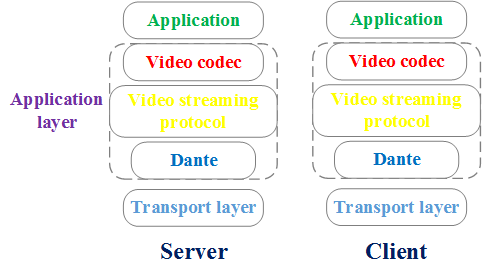
\includegraphics[scale=0.4]{paper_figs/stack_dante.png}
	\caption{Illustration Of Dante}
	\label{paper_figs:pathdemo}
\end{figure}

\begin{figure}[ht]
	\centering
	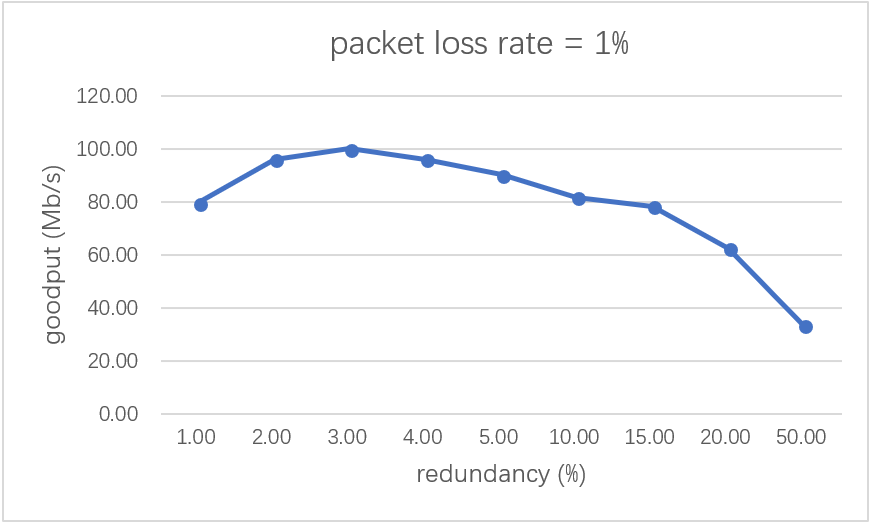
\includegraphics[scale=0.25]{paper_figs/tradeoff_only_goodput.png}
	\caption{Illustration Of Dante}
	\label{paper_figs:pathdemo}
\end{figure}

